% Observer/Estimator
% Author: Dominik Haumann
\documentclass[landscape,a5paper,11pt]{article}
\usepackage[utf8x]{inputenc} % utf8 encoding
\usepackage[T1]{fontenc} % use T1 fonts
\usepackage{amsmath} % nice math symbols
\usepackage{bm} % bold math
\usepackage{color} % change text color   

\usepackage{tikz}
\usetikzlibrary{decorations.pathmorphing} % for snake lines
\usetikzlibrary{matrix} % for block alignment
\usetikzlibrary{arrows} % for arrow heads
\usetikzlibrary{calc} % for manimulation of coordinates
\usetikzlibrary{shapes}
\usetikzlibrary{positioning}

% TikZ styles for drawing
\tikzstyle{block} = [draw, fill=white, rectangle, 
minimum height=3em, minimum width=6em]
\tikzstyle{sum} = [draw, fill=white, circle, node distance=1cm]
\tikzstyle{point} = [coordinate]
\tikzstyle{output} = [coordinate]
\tikzstyle{pinstyle} = [pin edge={to-,thin,black}]
\usetikzlibrary{positioning}

\renewcommand{\vec}[1]{\ensuremath{\boldsymbol{#1}}} % bold vectors
\def \myneq {\skew{-2}\not =} % \neq alone skews the dash

\begin{document}
	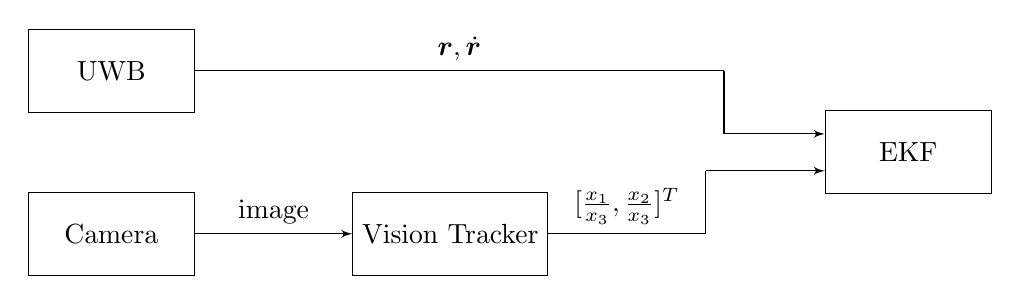
\begin{tikzpicture}[auto, node distance=2cm,>=latex']
		\node [block] (uwb) {UWB};
		\node [point] (p1) [right= 6.72cm of uwb]{};
		\node [point] (p2) [below= 0.8cm of p1]{};
		
		\node [block] (camera) [below = 1cm of uwb] {Camera};	
		\node [block] (visionTracker) [right=2cm of camera] {Vision Tracker};
		\node [point] (p3) [right= 2.0cm of visionTracker]{};
		\node [point] (p4) [above = 0.8cm of p3]{};
		
		
		
		\node [block] (ekf) [below right =-0.04cm and 8cm of uwb] {EKF};
		
		\draw [-] (uwb) -- node[name=u] {$\vec r, \dot{\vec r}$} (p1);
		\draw [-] (p1) -- node[name=u] {} (p2);
		
		\draw [-] (visionTracker) -- node[name=u] {$[\frac{x_1}{x_3}, \frac{x_2}{x_3}]^T$} (p3);
		\draw [-] (p3) -- node[name=u] {} (p4);
		
		\draw [->] (p2) -- node[name=u] {} (p2-|ekf.west);
		\draw [->] (p4) -- node[name=u] {} (p4-|ekf.west);
		
		\draw [->] (camera) -- node[name=u] {image} (visionTracker);
	
	%\node [block, above right of=visionTracker, name=ekf , above right=0.7cm and 4cm of uwb] {EKF};
%	
%	\node [input, name=input] {};
%	\node [sum, right of=input] (sum) {};
%	\node [block, right of=sum] (controller) {Controller};
%	\node [block, right of=controller, pin={[pinstyle]above:D},
%	node distance=3cm] (system) {System};
%	
%	\draw [->] (controller) -- node[name=u] {$u$} (system);
%	\node [output, right of=system] (output) {};
%	%\node [block, below of=u] (measurements) {Measurements};
%	\coordinate [below of=u] (measurements) {};
%	
%	\draw [draw,->] (input) -- node {$r$} (sum);
%	\draw [->] (sum) -- node {$e$} (controller);
%	\draw [->] (system) -- node [name=y] {$y$}(output);
%	%\draw [->] (y) |- (measurements);
%	\draw [-] (y) |- (measurements);
%	%\draw [->] (measurements) -| node[pos=0.99] {$-$} 
%	\draw [->] (measurements) -| %node[pos=1.00] {$-$} 
%	node [near end] {$y_m$} (sum);
%	
	%\draw [->] 

	\end{tikzpicture}
\end{document}